% Gabarit pandoc des corrigés publiés (brut et guidé). Contenu sans marque ni nom de site.
% Compilation : lualatex (latexmk -lualatex).
% Le Markdown reste la source unique : ne pas éditer ce fichier .tex à la main.
\documentclass[11pt,a4paper]{article}

% --- Moteur, polices (Latin Modern) et langue ---------------------------------
\usepackage{iftex}
\ifLuaTeX\else\errmessage{Ce document se compile avec lualatex}\fi
\usepackage{amsmath,amssymb,mathtools}
\usepackage{fontspec}
% mathrm=sym : \mathrm prend ses glyphes dans la police mathématique (ℓ, μ, Ω), comme KaTeX.
\usepackage[math-style=TeX,bold-style=TeX,mathrm=sym]{unicode-math}
% Repli pour les glyphes absents de Latin Modern (indices et exposants Unicode,
% flèches, filets des schémas en texte, symboles) : DejaVu, puis Latin Modern Math
% (ℓ, lettres mathématiques Unicode des légendes).
\directlua{
  luaotfload.add_fallback("repliTexte", {"DejaVuSerif:mode=harf;", "DejaVuSans:mode=harf;", "file:latinmodern-math.otf:mode=harf;"})
  luaotfload.add_fallback("repliMono", {"DejaVuSansMono:mode=harf;", "DejaVuSans:mode=harf;", "file:latinmodern-math.otf:mode=harf;"})
}
\setmainfont{Latin Modern Roman}[RawFeature={fallback=repliTexte}]
\setsansfont{Latin Modern Sans}[RawFeature={fallback=repliTexte}]
\setmonofont{Latin Modern Mono}[RawFeature={fallback=repliMono}]
\setmathfont{Latin Modern Math}
\usepackage[french]{babel}
\frenchsetup{SmallCapsFigTabCaptions=false}

% --- Mise en page --------------------------------------------------------------
\usepackage[a4paper,margin=2.2cm,headheight=14pt,footskip=1.2cm]{geometry}
\usepackage{microtype}
\setlength{\emergencystretch}{4em}
\tolerance=1500
\setlength{\parindent}{0pt}
\setlength{\parskip}{0.55\baselineskip plus 2pt minus 1pt}
\usepackage{xcolor}
% Gris nommés : babel-french rend « ! » actif dans le document.
\definecolor{gris2}{gray}{0.98}
\definecolor{gris3}{gray}{0.97}
\definecolor{gris5}{gray}{0.95}
\definecolor{gris35}{gray}{0.65}
\definecolor{gris40}{gray}{0.60}
\definecolor{gris45}{gray}{0.55}
\definecolor{gris50}{gray}{0.50}
\definecolor{gris55}{gray}{0.45}
\definecolor{gris60}{gray}{0.40}
\definecolor{gris65}{gray}{0.35}
\definecolor{gris70}{gray}{0.30}
\definecolor{gris80}{gray}{0.20}
\definecolor{gris85}{gray}{0.15}
\usepackage{graphicx}
\usepackage{float}
\usepackage{caption}
\captionsetup{font=small,labelformat=empty,justification=centering}
\usepackage{booktabs,longtable,array,multirow,calc}
\usepackage{siunitx}
\sisetup{locale=FR}
\usepackage[version=4]{mhchem}
\usepackage{listings}
\usepackage{fancyhdr}
\usepackage{lastpage}
\usepackage[most]{tcolorbox}
\usepackage{enumitem}
\setlist{nosep,leftmargin=*,topsep=2pt}
\usepackage[hidelinks,unicode]{hyperref}
\usepackage{bookmark}
\hypersetup{pdftitle={Mines-Ponts MPI — Informatique 2 2026},pdfauthor={Rédigé par IA},pdfcreator={LaTeX},pdfsubject={Corrigé brut}}
\usepackage{xurl}

% --- Pandoc : listes, tableaux, figures ----------------------------------------
\providecommand{\passthrough}[1]{#1}
\providecommand{\tightlist}{\setlength{\itemsep}{0pt}\setlength{\parskip}{0pt}}

\makeatletter
\def\maxwidth{\ifdim\Gin@nat@width>\linewidth\linewidth\else\Gin@nat@width\fi}
\def\maxheight{\ifdim\Gin@nat@height>0.55\textheight 0.55\textheight\else\Gin@nat@height\fi}
\makeatother
\setkeys{Gin}{width=\maxwidth,height=\maxheight,keepaspectratio}
\setcounter{secnumdepth}{-\maxdimen}
\providecommand{\pandocbounded}[1]{#1}
\usepackage{longtable,booktabs,array}

% --- Code (listings) -----------------------------------------------------------
\lstset{
  basicstyle=\ttfamily\small,
  columns=fullflexible,
  keepspaces=true,
  breaklines=true,
  breakatwhitespace=false,
  postbreak=\mbox{\textcolor{gris50}{$\hookrightarrow$}\space},
  frame=single,
  rulecolor=\color{gris35},
  framesep=4pt,
  xleftmargin=5pt,xrightmargin=5pt,
  backgroundcolor=\color{gris3},
  keywordstyle=\bfseries,
  commentstyle=\color{gris65},
  stringstyle=\color{gris80},
  showstringspaces=false,
  tabsize=4,
  extendedchars=true,
  aboveskip=6pt,belowskip=6pt,
}

% --- Macros des corrigés (KaTeX ↔ LaTeX) ---------------------------------------
% Les corrigés sont écrits pour KaTeX : on définit ici ce que KaTeX connaît et
% que LaTeX n'a pas, sans jamais retoucher le Markdown.
\providecommand{\R}{\mathbb{R}}
\providecommand{\N}{\mathbb{N}}
\providecommand{\Z}{\mathbb{Z}}
\providecommand{\Q}{\mathbb{Q}}
\providecommand{\C}{\mathbb{C}}
\providecommand{\dd}{\mathrm{d}}
\providecommand{\llbracket}{\lBrack}
\providecommand{\rrbracket}{\rBrack}
\providecommand{\lBrace}{\lbrace}
\providecommand{\rBrace}{\rbrace}
\providecommand{\Box}{\square}
\providecommand{\Diamond}{\lozenge}
\providecommand{\varnothing}{\emptyset}
\providecommand{\argmax}{\operatorname*{arg\,max}}
\providecommand{\argmin}{\operatorname*{arg\,min}}
\renewcommand{\leq}{\leqslant}
\renewcommand{\geq}{\geqslant}

% Équation hors texte : réduite à la largeur de la ligne si elle déborde.
\newsavebox{\boiteequation}
\newcommand{\equationajustee}[1]{%
  \sbox{\boiteequation}{$\displaystyle #1$}%
  \ifdim\wd\boiteequation>\linewidth
    \[\resizebox{\linewidth}{!}{\usebox{\boiteequation}}\]%
  \else
    \[#1\]%
  \fi}

% --- Encadrés pédagogiques (sobres, lisibles en noir et blanc) -----------------
\tcbset{
  encadre/.style={
    enhanced,breakable,sharp corners,
    colback=white,colframe=gris55,
    boxrule=0.4pt,leftrule=2.2pt,
    left=6pt,right=6pt,top=3pt,bottom=3pt,
    before skip=6pt,after skip=6pt,
    fonttitle=\bfseries\small,coltitle=black,
    attach title to upper,after title={\quad},
    parbox=false,
  }
}
\newtcolorbox{indication}[1]{encadre,colframe=gris45,colback=gris2,title={Indication~#1}}
\newtcolorbox{methode}{encadre,colframe=gris70,title={Méthode}}
\newtcolorbox{piege}{encadre,colframe=gris85,boxrule=0.8pt,leftrule=2.2pt,title={Piège}}
\newtcolorbox{jury}{encadre,colframe=gris60,colback=gris5,title={Jury}}
\newtcolorbox{encadrenote}{encadre,colframe=gris40}

% --- Titres de section ---------------------------------------------------------
\usepackage{titlesec}
\titleformat{\section}{\Large\bfseries}{}{0pt}{}
\titleformat{\subsection}{\large\bfseries}{}{0pt}{}
\titleformat{\subsubsection}{\normalsize\bfseries}{}{0pt}{}
\titlespacing*{\section}{0pt}{14pt plus 4pt minus 2pt}{6pt}
\titlespacing*{\subsection}{0pt}{10pt plus 3pt minus 2pt}{4pt}
\titlespacing*{\subsubsection}{0pt}{8pt plus 2pt minus 2pt}{2pt}

% --- En-tête et pied de page ---------------------------------------------------
\pagestyle{fancy}
\fancyhf{}
\fancyhead[L]{\small\textsc{Corrigé brut} · Mines-Ponts MPI}
\fancyhead[R]{\small Informatique 2 2026}
\fancyfoot[L]{\footnotesize Corrigé rédigé par IA, non officiel}
\fancyfoot[R]{\footnotesize \thepage\,/\,\pageref*{LastPage}}
\renewcommand{\headrulewidth}{0.4pt}
\renewcommand{\footrulewidth}{0pt}
\fancypagestyle{plain}{\fancyhf{}\fancyfoot[R]{\footnotesize \thepage\,/\,\pageref*{LastPage}}\fancyfoot[L]{\footnotesize Corrigé rédigé par IA, non officiel}\renewcommand{\headrulewidth}{0pt}}

\begin{document}
\thispagestyle{plain}
\begin{center}
  {\small\scshape Corrigé brut}\par\smallskip
  {\LARGE\bfseries Mines-Ponts MPI — Informatique 2 2026\par}\medskip
  {\large Mines-Ponts · MPI · Informatique 2 · 2026\par}
\end{center}
\vspace{2pt}\hrule\vspace{8pt}

\emph{Corrigé rédigé par IA, non officiel. Signalez toute erreur.}

Épreuve de 4 heures, calculatrice et tout dispositif électronique interdits. Langage C pour la programmation (en-têtes \texttt{assert.h}, \texttt{stdbool.h}, \texttt{stddef.h}, \texttt{stdint.h}, \texttt{stdio.h}, \texttt{stdlib.h}, \texttt{string.h} supposés inclus), SQL pour les requêtes. 38 questions.

Notations : \(n_s\) (ou \texttt{ns}) nombre de salles, \(n_p\) (ou \texttt{np}) nombre de passages, \(\delta(u,v)\) coût minimal d'un chemin de \(u\) à \(v\), \(c(u,v)\) coût d'un passage.

\hypertarget{repruxe9sentation-relationnelle-des-donnuxe9es}{%
\section{1 Représentation relationnelle des données}\label{repruxe9sentation-relationnelle-des-donnuxe9es}}

\hypertarget{question-1}{%
\subsection{Question 1}\label{question-1}}

Une salle contient zéro, un ou plusieurs objets ; un objet est posé dans exactement une salle. L'association « objet est placé dans salle » est donc de type \textbf{un-à-plusieurs} : cardinalité \((1,1)\) du côté \texttt{objet} (chaque objet référence une et une seule salle) et \((0,N)\) du côté \texttt{salle} (une salle est référencée par un nombre quelconque d'objets).

Un attribut relationnel est atomique : il ne contient qu'une valeur. La clé étrangère doit donc être placée dans la table dont chaque ligne ne référence qu'\textbf{une} ligne de l'autre table, c'est-à-dire \texttt{objet}. Un attribut \texttt{objet\_id} dans \texttt{salle} serait mal formé :

\begin{itemize}
\tightlist
\item
  une salle contenant \(k \ge 2\) objets demanderait \(k\) valeurs dans un même attribut (violation de l'atomicité), ou bien \(k\) lignes pour la même salle, ce qui casse l'unicité de la clé primaire \texttt{salle.id} et duplique \texttt{nom}, \texttt{x}, \texttt{y} (redondance, risque d'incohérence) ;
\item
  une salle vide devrait porter une valeur \texttt{NULL}.
\end{itemize}

\textbf{La clé étrangère \texttt{salle\_id} est dans \texttt{objet} car l'association est de cardinalité 1--∗ (1--N) : un objet appartient à une seule salle, une salle contient 0 à N objets.}

\hypertarget{question-2}{%
\subsection{Question 2}\label{question-2}}

\begin{lstlisting}[language=SQL]
SELECT DISTINCT arr.nom
FROM passage AS p
JOIN salle AS dep ON p.entree = dep.id
JOIN salle AS arr ON p.sortie = arr.id
WHERE dep.nom = 'ENTRÉE';
\end{lstlisting}

La table \texttt{salle} apparaît deux fois (alias \texttt{dep} pour la salle de départ, \texttt{arr} pour la salle d'arrivée). \texttt{DISTINCT} évite les doublons si plusieurs passages relient les deux mêmes salles.

\hypertarget{question-3}{%
\subsection{Question 3}\label{question-3}}

\begin{lstlisting}[language=SQL]
SELECT s.nom, COUNT(p.id) AS nb_sortants
FROM salle AS s
LEFT JOIN passage AS p ON p.entree = s.id
GROUP BY s.id, s.nom;
\end{lstlisting}

« Pour chaque salle » impose la jointure externe : une salle sans passage sortant doit apparaître avec 0. \texttt{COUNT(p.id)} ignore les \texttt{NULL} produits par la jointure externe, alors que \texttt{COUNT(*)} donnerait 1 pour une telle salle. On regroupe sur la clé \texttt{s.id} (deux salles peuvent porter le même nom).

\hypertarget{question-4}{%
\subsection{Question 4}\label{question-4}}

\begin{lstlisting}[language=SQL]
SELECT s.nom, MIN(p.cout) AS cout_min
FROM salle AS s
JOIN passage AS p ON p.entree = s.id
GROUP BY s.id, s.nom
ORDER BY cout_min DESC, s.nom ASC;
\end{lstlisting}

La jointure interne ne conserve que les salles possédant au moins un passage sortant, ce qui est exactement la restriction demandée.

\hypertarget{question-5}{%
\subsection{Question 5}\label{question-5}}

\begin{lstlisting}[language=SQL]
SELECT s.nom, COUNT(o.id) AS nb_objets
FROM salle AS s
JOIN objet AS o ON o.salle_id = s.id
GROUP BY s.id, s.nom
HAVING COUNT(o.id) >= 2;
\end{lstlisting}

Le filtre porte sur un agrégat : il se place dans \texttt{HAVING}, pas dans \texttt{WHERE}. Les salles sans objet sont de toute façon éliminées par ce filtre, la jointure interne suffit.

\hypertarget{repruxe9sentation-en-muxe9moire-et-navigation-dans-le-monde}{%
\section{2 Représentation en mémoire et navigation dans le monde}\label{repruxe9sentation-en-muxe9moire-et-navigation-dans-le-monde}}

\hypertarget{impluxe9mentation-classique-du-graphe-ponduxe9ruxe9}{%
\subsection{2.1 Implémentation classique du graphe pondéré}\label{impluxe9mentation-classique-du-graphe-ponduxe9ruxe9}}

\hypertarget{question-6}{%
\subsection{Question 6}\label{question-6}}

\begin{lstlisting}[language=C]
monde* monde_init(int n) {
    assert(n >= 0);
    monde* m = malloc(sizeof(monde));
    assert(m != NULL);
    m->taille = n;
    m->salles = malloc(n * sizeof(salle*));
    assert(n == 0 || m->salles != NULL);
    for (int i = 0; i < n; i++) {
        m->salles[i] = malloc(sizeof(salle));
        assert(m->salles[i] != NULL);
        m->salles[i]->id = i;              /* id = indice dans le tableau */
        m->salles[i]->passages = NULL;     /* liste de passages vide */
    }
    return m;
}
\end{lstlisting}

On alloue la structure, le tableau de \(n\) pointeurs, puis les \(n\) salles. Le test \texttt{n\ ==\ 0\ \textbar{}\textbar{}} tient compte de ce que \texttt{malloc(0)} peut renvoyer \texttt{NULL}. Complexité \(O(n)\).

\hypertarget{question-7}{%
\subsection{Question 7}\label{question-7}}

\begin{lstlisting}[language=C]
int monde_degre(monde* m, int s) {
    assert(m != NULL && 0 <= s && s < m->taille);
    int d = 0;
    for (passage* p = m->salles[s]->passages; p != NULL; p = p->suivant) {
        d++;
    }
    return d;
}
\end{lstlisting}

Complexité \(O(d^+(s))\).

\hypertarget{question-8}{%
\subsection{Question 8}\label{question-8}}

\begin{lstlisting}[language=C]
int monde_sommeDegres(monde* m) {
    assert(m != NULL);
    int total = 0;
    for (int s = 0; s < m->taille; s++) {
        total += monde_degre(m, s);
    }
    return total;
}
\end{lstlisting}

Chaque passage est sortant d'exactement une salle et figure une seule fois dans la liste de celle-ci : la somme des degrés sortants vaut \(n_p\). Complexité \(O(n_s + n_p)\).

\hypertarget{question-9}{%
\subsection{Question 9}\label{question-9}}

\begin{lstlisting}[language=C]
int monde_coutTotal(monde* m) {
    assert(m != NULL);
    int total = 0;
    for (int s = 0; s < m->taille; s++) {
        for (passage* p = m->salles[s]->passages; p != NULL; p = p->suivant) {
            total += p->cout;
        }
    }
    return total;
}
\end{lstlisting}

Complexité \(O(n_s + n_p)\). (Sur un très grand monde, la somme pourrait dépasser la capacité d'un \texttt{int} ; un \texttt{int64\_t} lèverait ce risque.)

\hypertarget{question-10}{%
\subsection{Question 10}\label{question-10}}

Entiers et pointeurs occupent 4 octets ; tous les champs ayant même taille et même alignement, il n'y a pas d'octet de remplissage. On ne compte pas le surcoût interne de l'allocateur.

\begin{itemize}
\tightlist
\item
  \texttt{monde} : \texttt{salles} + \texttt{taille} = 8 octets, une fois ;
\item
  tableau \texttt{salles} : \(n_s\) pointeurs, soit \(4n_s\) octets ;
\item
  \texttt{salle} : \texttt{id} + \texttt{passages} = 8 octets, \(n_s\) fois ;
\item
  \texttt{passage} : \texttt{cout} + \texttt{sortie} + \texttt{suivant} = 12 octets, \(n_p\) fois (chaque passage n'est stocké que dans la liste de sa salle d'entrée).
\end{itemize}

\equationajustee{\boxed{M_{\text{listes}} = 8 + 4n_s + 8n_s + 12n_p = 12\,n_s + 12\,n_p + 8 \ \text{octets}}}

\hypertarget{question-11}{%
\subsection{Question 11}\label{question-11}}

Avec \(n_p \approx 4n_s\) : \(M_{\text{listes}} \approx 12n_s + 48n_s = 60\,n_s\) octets. La mémoire disponible est \(64 \text{ Ko} = 65\,536\) octets, d'où \(n_s \lesssim 65\,536/60 \approx 1\,100\).

\textbf{L'ordre de grandeur plausible est 1 000 salles.} (Le surcoût réel des \(n_s + n_p + 2\) blocs alloués ne peut que diminuer cette valeur, ce qui exclut 10 000.)

\hypertarget{repruxe9sentation-csr-pour-un-graphe}{%
\subsection{2.2 Représentation CSR pour un graphe}\label{repruxe9sentation-csr-pour-un-graphe}}

\hypertarget{question-12}{%
\subsection{Question 12}\label{question-12}}

\texttt{indices} a 6 cases, donc \(n_s = 5\) salles (0 à 4) ; la sentinelle \texttt{indices{[}5{]}\ =\ 7} donne \(n_p = 7\). Les tranches \([\![\texttt{indices[s]}, \texttt{indices[s+1]}-1]\!]\) donnent :

\begin{longtable}[]{@{}lll@{}}
\toprule\noalign{}
salle \(s\) & cases \(k\) & passages (coût) \\
\midrule\noalign{}
\endhead
\bottomrule\noalign{}
\endlastfoot
0 & 0, 1 & \(0 \to 1\) (2), \(0 \to 3\) (5) \\
1 & 2 & \(1 \to 2\) (1) \\
2 & 3, 4 & \(2 \to 0\) (4), \(2 \to 4\) (3) \\
3 & 5 & \(3 \to 1\) (6) \\
4 & 6 & \(4 \to 2\) (2) \\
\end{longtable}

Le graphe orienté pondéré a 5 sommets et 7 arcs (figure 1).

\begin{figure}[H]
\centering
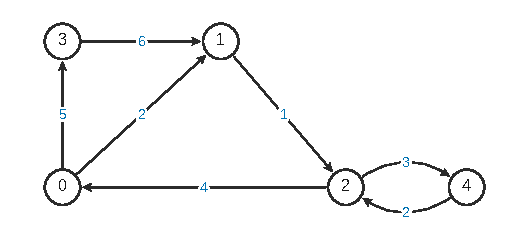
\includegraphics{figures/q12-graphe-csr.pdf}
\caption*{Figure 1 --- Graphe orienté pondéré codé par la représentation CSR de la
question 12 : 5 salles, 7 passages, coût porté sur chaque arc}
\end{figure}

Les arcs \(2 \to 4\) (coût 3) et \(4 \to 2\) (coût 2) sont deux passages distincts. Le graphe est fortement connexe (circuits \(0\to1\to2\to0\), \(0\to3\to1\), \(2\to4\to2\)).

\hypertarget{question-13}{%
\subsection{Question 13}\label{question-13}}

\begin{lstlisting}[language=C]
mondeCSR* mondeCSR_init(int ns, int np) {
    assert(ns >= 0 && np >= 0);
    mondeCSR* mc = malloc(sizeof(mondeCSR));
    assert(mc != NULL);
    mc->nb_salles = ns;
    mc->indices = malloc((ns + 1) * sizeof(int));   /* sentinelle incluse */
    mc->sorties = malloc(np * sizeof(int));
    mc->couts   = malloc(np * sizeof(int));
    assert(mc->indices != NULL);
    assert(np == 0 || (mc->sorties != NULL && mc->couts != NULL));
    return mc;
}
\end{lstlisting}

\hypertarget{question-14}{%
\subsection{Question 14}\label{question-14}}

\begin{lstlisting}[language=C]
int mondeCSR_degre(mondeCSR* mc, int s) {
    assert(mc != NULL && 0 <= s && s < mc->nb_salles);
    return mc->indices[s + 1] - mc->indices[s];
}
\end{lstlisting}

La tranche de \(s\) a \(\texttt{indices[s+1]} - \texttt{indices[s]}\) cases ; l'accès à \texttt{indices{[}s+1{]}} est licite car \(s + 1 \le n_s\) (sentinelle). Complexité \(O(1)\).

\hypertarget{question-15}{%
\subsection{Question 15}\label{question-15}}

\begin{lstlisting}[language=C]
int mondeCSR_sommeDegres(mondeCSR* mc) {
    assert(mc != NULL);
    return mc->indices[mc->nb_salles];   /* sentinelle : vaut np */
}
\end{lstlisting}

La somme des degrés se télescope, et \texttt{indices{[}0{]}} vaut 0 :

\equationajustee{\begin{aligned}
\sum_{s=0}^{n_s-1}\left(\texttt{indices}[s+1] - \texttt{indices}[s]\right)
&= \texttt{indices}[n_s] - \texttt{indices}[0] \\
&= \texttt{indices}[n_s] = n_p .
\end{aligned}}

Aucune boucle n'est nécessaire : complexité \(O(1)\).

\hypertarget{question-16}{%
\subsection{Question 16}\label{question-16}}

\begin{lstlisting}[language=C]
int mondeCSR_coutTotal(mondeCSR* mc) {
    assert(mc != NULL);
    int np = mc->indices[mc->nb_salles];   /* nombre total de passages */
    int total = 0;
    for (int k = 0; k < np; k++) {
        total += mc->couts[k];
    }
    return total;
}
\end{lstlisting}

Les tranches partitionnent \([\![0, n_p - 1]\!]\) : un parcours linéaire de \texttt{couts} suffit. Complexité \(O(n_p)\).

\hypertarget{question-17}{%
\subsection{Question 17}\label{question-17}}

\begin{lstlisting}[language=C]
mondeCSR* monde_vers_CSR(monde* m) {
    assert(m != NULL);
    int ns = m->taille;
    int np = monde_sommeDegres(m);
    mondeCSR* mc = mondeCSR_init(ns, np);
    int k = 0;
    for (int s = 0; s < ns; s++) {
        mc->indices[s] = k;                     /* début de la tranche de s */
        for (passage* p = m->salles[s]->passages; p != NULL; p = p->suivant) {
            mc->sorties[k] = p->sortie;
            mc->couts[k] = p->cout;
            k++;
        }
    }
    mc->indices[ns] = k;                        /* sentinelle : k = np */
    return mc;
}
\end{lstlisting}

L'allocation passe par \texttt{mondeCSR\_init}, et la première itération pose \texttt{indices{[}0{]}\ =\ 0}.

Invariant : avant le traitement de la salle \(s\), les cases \(0\) à \(k-1\) contiennent, dans l'ordre, les passages des salles \(0\) à \(s-1\). De plus, \texttt{indices{[}j{]}} est correct pour tout \(j < s\).

En fin de boucle, \(k = n_p\), valeur de la sentinelle. Complexité \(O(n_s + n_p)\) ; \texttt{m} n'est pas modifié.

\hypertarget{question-18}{%
\subsection{Question 18}\label{question-18}}

\texttt{mondeCSR} contient trois pointeurs et un entier : 16 octets. Tableaux : \texttt{indices} \(4(n_s + 1)\), \texttt{sorties} \(4n_p\), \texttt{couts} \(4n_p\).

\equationajustee{\boxed{M_{\text{CSR}} = 16 + 4(n_s+1) + 8n_p = 4\,n_s + 8\,n_p + 20 \ \text{octets}}}

\hypertarget{question-19}{%
\subsection{Question 19}\label{question-19}}

Les deux occupations (questions 10 et 18) sont :

\equationajustee{\begin{aligned}
M_{\text{listes}} &= 12\,n_s + 12\,n_p + 8, \\
M_{\text{CSR}} &= 4\,n_s + 8\,n_p + 20 .
\end{aligned}}

Leur différence vaut :

\equationajustee{\begin{aligned}
M_{\text{listes}} - M_{\text{CSR}}
&= (12\,n_s + 12\,n_p + 8) - (4\,n_s + 8\,n_p + 20) \\
&= 8\,n_s + 4\,n_p - 12 .
\end{aligned}}

Elle est strictement positive dès que \(2n_s + n_p \ge 4\), donc pour tout monde non trivial.

Coefficient par coefficient : par salle, on passe de 12 à 4 octets (plus de structure \texttt{salle} ni de pointeur vers elle) ; par passage, de 12 à 8 octets (le pointeur \texttt{suivant} disparaît grâce à la contiguïté).

Avec \(n_p = 4n_s\), on compare \(60\,n_s\) à \(36\,n_s\) : rapport \(5/3\), soit environ 40 \% d'économie. Dans 64 Ko, on passe d'environ 1 100 à environ 1 800 salles.

\textbf{Conclusion : la représentation CSR est toujours plus compacte.} Elle demande en outre 4 allocations au lieu de \(n_s + n_p + 2\) (moins de surcoût d'allocateur), offre un accès séquentiel aux passages d'une salle (bonne localité) et un degré en \(O(1)\). Contrepartie : c'est une structure statique (ajouter un passage coûte \(O(n_s + n_p)\)), adaptée à un monde figé au chargement du niveau.

\hypertarget{recherche-dun-chemin-de-couxfbt-minimal}{%
\subsection{2.3 Recherche d'un chemin de coût minimal}\label{recherche-dun-chemin-de-couxfbt-minimal}}

\hypertarget{question-20}{%
\subsection{Question 20}\label{question-20}}

Le parcours en largeur depuis \(s\) utilise une file. On enfile \(s\) marqué ; puis on défile un sommet \(u\) et on enfile, en les marquant, ses successeurs non marqués, en retenant \(u\) comme père.

Notons \(\ell(t)\) le nombre minimal de passages d'un chemin de \(s\) à \(t\), et \(\mathrm{niv}(t)\) la longueur du chemin de \(s\) à \(t\) dans l'arbre des pères.

\begin{itemize}
\tightlist
\item
  \textbf{Invariant de la file.} Les niveaux des sommets de la file sont croissants au sens large et prennent au plus deux valeurs consécutives \(d\) et \(d+1\). C'est vrai pour la file \((s)\). Défiler un sommet de niveau \(d\) et enfiler en queue des sommets de niveau \(d+1\) le conserve. Les sommets sont donc marqués \textbf{par couches}, de niveaux croissants.
\item
  \textbf{Récurrence sur \(d\).} Montrons que tout \(t\) tel que \(\ell(t) = d\) est marqué au niveau \(d\). Pour \(d = 0\), \(t = s\).
\item
  Pour \(d \ge 1\), soit \(s \to \dots \to v \to t\) un chemin de \(d\) passages. Alors \(\ell(v) = d - 1\), donc \(v\) est marqué au niveau \(d-1\) par hypothèse de récurrence.
\item
  Quand \(v\) est défilé, ou bien \(t\) est marqué à cet instant, au niveau \(d\), ou bien il est déjà marqué. Dans ce second cas, son niveau est au plus \(d\), par le marquage par couches.
\item
  Ce niveau est aussi au moins \(\ell(t)\), car \(\mathrm{niv}(t)\) est la longueur d'un vrai chemin. Il vaut donc \(d\).
\end{itemize}

Le chemin de l'arbre des pères de \(s\) à \(t\) utilise donc \textbf{un nombre minimal de passages}, et tout \(t\) est atteint car le graphe est fortement connexe.

\textbf{Cas où ces chemins sont de coût minimal : tous les passages ont le même coût \(c > 0\).} Le coût d'un chemin vaut alors \(c\) fois son nombre de passages, fonction strictement croissante du nombre de passages. (C'est aussi le cas, trivialement, si chaque salle n'est reliée à \(s\) que par un seul chemin élémentaire, par exemple un graphe en arbre.)

\hypertarget{question-21}{%
\subsection{Question 21}\label{question-21}}

\begin{lstlisting}[language=C]
int* bfs_cout(mondeCSR* mc, int s) {
    assert(mc != NULL && 0 <= s && s < mc->nb_salles);
    int n = mc->nb_salles;
    int* dist = malloc(n * sizeof(int));
    assert(dist != NULL);
    for (int u = 0; u < n; u++) { dist[u] = -1; }   /* -1 : salle non atteinte */
    file* f = file_init(n);                  /* chaque salle enfilée au plus une fois */
    dist[s] = 0;
    file_enfile(f, s);
    while (!file_vide(f)) {
        int u = file_defile(f);
        for (int k = mc->indices[u]; k < mc->indices[u + 1]; k++) {
            int v = mc->sorties[k];
            if (dist[v] == -1) {             /* v découverte maintenant */
                dist[v] = dist[u] + mc->couts[k];
                file_enfile(f, v);
            }
        }
    }
    file_libere(f);
    return dist;                             /* à libérer par l'appelant */
}
\end{lstlisting}

La valeur \(-1\) sert de marque « non atteinte » : une salle atteinte a une valeur \(\ge 0\) (0 pour \(s\), et les coûts sont strictement positifs). Une initialisation à 0 ne permettrait pas de distinguer une salle non atteinte de la source. Aucun autre tableau n'est nécessaire.

La marque est posée à l'enfilement. Une salle est donc enfilée au plus une fois (la capacité \(n\) suffit), et \texttt{dist{[}v{]}} est écrit une seule fois : c'est le coût du chemin de l'arbre du parcours. Le graphe étant fortement connexe, aucune case ne reste à \(-1\). Complexité \(O(n_s + n_p)\).

\hypertarget{question-22}{%
\subsection{Question 22}\label{question-22}}

Par récurrence sur l'ordre de découverte, \texttt{dist{[}u{]}} est le coût d'un chemin effectif \(P_u\) de \(s\) à \(u\), celui de l'arbre du parcours. En effet \texttt{dist{[}s{]}\ =\ 0}, et \texttt{dist{[}v{]}\allowbreak{}\ =\allowbreak{}\ dist{[}u{]}\allowbreak{}\ +\ c(\allowbreak{}u,\allowbreak{}v)\allowbreak{}} quand \(v\) est découverte depuis \(u\).

Le coût minimal \(\delta(s,u)\) est le minimum des coûts des chemins de \(s\) à \(u\). Ce minimum existe : l'ensemble des chemins est non vide (forte connexité) et, les coûts étant strictement positifs, on peut se restreindre aux chemins élémentaires, en nombre fini. Comme \(P_u\) est l'un de ces chemins :

\equationajustee{\delta(s,u) \le \mathrm{cout}(P_u) = \texttt{dist}[u].}

\textbf{\texttt{dist{[}u{]}} est donc un majorant du coût minimal.} Il peut être très mauvais : avec \(0 \to 2\) de coût \(M\) et \(0 \to 1 \to 2\) de coûts \(1, 1\), on obtient \(\texttt{dist}[2] = M\) alors que \(\delta(0,2) = 2\).

\hypertarget{question-23}{%
\subsection{Question 23}\label{question-23}}

Le tas ne propose pas de diminution de priorité : on ré-empile une salle à chaque amélioration et on ignore les entrées périmées grâce à un tableau \texttt{traite}.

Point essentiel : \texttt{dist} est initialisé par des valeurs finies, et non par \(+\infty\). \textbf{Toutes les salles doivent alors être empilées au départ}, avec leur priorité \texttt{dist{[}u{]}}, si la relaxation est stricte.

Si l'on n'empilait que \(s\), une salle \(v\) dont la valeur issue du parcours en largeur est déjà optimale ne serait jamais améliorée, donc jamais empilée ; ses successeurs ne seraient jamais relâchés depuis elle.

Exemple : passages \(0 \to 1\) (1), \(1 \to 2\) (1), \(0 \to 2\) (5) et \(2 \to 0\) (1). Le parcours en largeur donne \(\texttt{dist} = (0, 1, 5)\).

En n'empilant que 0, on relâche \(0 \to 1\) (test \(1 < 1\) faux), puis \(0 \to 2\) (test \(5 < 5\) faux). Le tas se vide, et \(\texttt{dist}[2]\) reste à 5 au lieu de 2 (figure 2).

\begin{figure}[H]
\centering
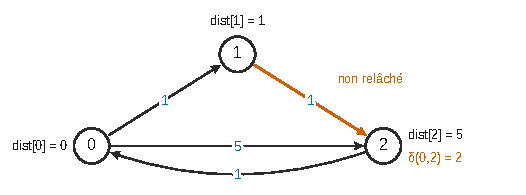
\includegraphics{figures/q23-contre-exemple-dijkstra.pdf}
\caption*{Figure 2 --- Contre-exemple de la question 23 : valeurs initiales de
bfs\_cout ; si l'on n'empile que 0, le passage 1→2 n'est jamais relâché
et la valeur de la salle 2 reste à 5 au lieu de 2}
\end{figure}

\begin{lstlisting}[language=C]
void dijkstra(mondeCSR* mc, int s, int* dist) {
    assert(mc != NULL && dist != NULL && 0 <= s && s < mc->nb_salles);
    int n = mc->nb_salles;
    bool* traite = malloc(n * sizeof(bool));
    assert(traite != NULL);
    tasMin* tm = tasMin_init();
    dist[s] = 0;
    for (int u = 0; u < n; u++) {           /* toutes les salles sont découvertes */
        traite[u] = false;
        tasMin_empile(tm, u, dist[u]);
    }
    while (!tasMin_vide(tm)) {
        int u = tasMin_depile(tm);
        if (!traite[u]) {                    /* sinon : entrée périmée */
            traite[u] = true;
            for (int k = mc->indices[u]; k < mc->indices[u + 1]; k++) {
                int v = mc->sorties[k];
                int d = dist[u] + mc->couts[k];
                if (d < dist[v]) {
                    dist[v] = d;
                    tasMin_empile(tm, v, d);
                }
            }
        }
    }
    tasMin_libere(tm);
    free(traite);
}
\end{lstlisting}

Variante tout aussi correcte : n'empiler que \(s\), mais relâcher avec un test large \texttt{d\ \textless{}=\allowbreak{}\ dist{[}v{]}\allowbreak{}\ \&\&\ !traite{[}v{]}\allowbreak{}}. Chaque salle est alors empilée au moins une fois, par récurrence le long de l'arbre du parcours en largeur. Seule la combinaison « source seule et test strict » est fausse.

\textbf{Correction.} Deux invariants valent à tout instant.

\begin{itemize}
\tightlist
\item
  (I1) \texttt{dist{[}u{]}} est le coût d'un chemin effectif, donc \(\texttt{dist}[u] \ge \delta(s,u)\) : vrai au départ (question 22), conservé par relâchement.
\item
  (I2) Toute salle non traitée a dans le tas une entrée de priorité égale à \texttt{dist{[}u{]}} : empilement initial, puis empilement à chaque diminution.
\end{itemize}

Les entrées d'une même salle ont des priorités décroissantes au fil des empilements. Le premier dépilement de \(u\) se fait donc avec la priorité \texttt{dist{[}u{]}} courante.

Supposons qu'une salle soit traitée avec une valeur non optimale, et soit \(u\) la première. Soit \(s = v_0, \dots, v_k = u\) un plus court chemin, et \(v_i\) sa première salle non traitée. On a \(i \ge 1\), car \(s\), seule de priorité 0, est traitée en premier.

Les \(v_j\) (\(j < i\)) ont été traitées avec leur valeur optimale et ont relâché \(v_j \to v_{j+1}\). D'où :

\equationajustee{\begin{aligned}
\texttt{dist}[v_i] &\le \delta(s,v_{i-1}) + c(v_{i-1},v_i) \\
&= \delta(s,v_i),
\end{aligned}}

donc égalité par (I1). Par (I2), le tas contient \(v_i\) avec la priorité \(\delta(s,v_i)\), et :

\equationajustee{\begin{aligned}
\delta(s,v_i) &\le \delta(s,u) \\
&< \texttt{dist}[u].
\end{aligned}}

Ce n'est donc pas \(u\) qui aurait été dépilée : contradiction. \textbf{À l'issue, \texttt{dist{[}u{]}} = \(\delta(s,u)\) pour toute salle \(u\).}

Complexité : au plus \(n_s + n_p\) entrées dans le tas, d'où \(O((n_s + n_p)\log(n_s + n_p))\).

\hypertarget{recherche-rapide-dun-chemin-avec-heuristique}{%
\section{3 Recherche rapide d'un chemin avec heuristique}\label{recherche-rapide-dun-chemin-avec-heuristique}}

\hypertarget{question-24}{%
\subsection{Question 24}\label{question-24}}

Notons \(f(u) = \texttt{dist}[u] + h(u)\) et \(\delta = \delta(s,t)\). \texttt{dist{[}u{]}} est toujours le coût d'un chemin effectif, donc \(\texttt{dist}[u] \ge \delta(s,u)\). Toute diminution de \texttt{dist{[}v{]}} provoque une (ré)insertion de \(v\).

\textbf{Lemme (sommet frontière).} Soit \(P = (s = v_0, \dots, v_k = t)\) un chemin optimal. À un instant où \(t\) est dans la file, soit \(v_i\) le sommet de \(P\) d'indice minimal présent dans la file. Alors \(\texttt{dist}[v_i] = \delta(s,v_i)\).

\emph{Preuve.} \(s\) a été extrait en premier, donc \(i \ge 1\). Pour \(j < i\), \(v_j\) n'est pas dans la file : depuis sa dernière modification de \texttt{dist}, il a été extrait et ses arcs relâchés.

Par récurrence sur \(j < i\), \(\texttt{dist}[v_j] = \delta(s,v_j)\). C'est vrai pour \(j = 0\). Si c'est vrai pour \(j\), la relaxation de \(v_j \to v_{j+1}\) donne :

\equationajustee{\begin{aligned}
\texttt{dist}[v_{j+1}] &\le \delta(s,v_j) + c(v_j,v_{j+1}) \\
&= \delta(s,v_{j+1}),
\end{aligned}}

car un préfixe de chemin optimal est optimal. Avec la minoration, il y a égalité, jusqu'à \(\texttt{dist}[v_i] = \delta(s,v_i)\).

\textbf{Preuve par l'absurde.} Supposons \(t\) extraite avec \(\texttt{dist}[t] > \delta\). Juste avant l'extraction, \(t\) est dans la file ; soit \(v_i\) le sommet frontière. Alors :

\equationajustee{\begin{aligned}
f(v_i) &= \delta(s,v_i) + h(v_i) \\
&\le \delta(s,v_i) + \delta(v_i,t) && \text{(\text{admissibilité})} \\
&= \delta && (v_i \text{ est sur un chemin optimal}) \\
&< \texttt{dist}[t] && \text{(\text{hypothèse})} \\
&= \texttt{dist}[t] + h(t) && (h(t) = 0) \\
&= f(t).
\end{aligned}}

Les salles étant extraites par valeur de \(f\) minimale, \(v_i\) (ou une salle de priorité encore plus faible) aurait été extraite avant \(t\) : contradiction.

\textbf{Donc, dès que \(t\) est extraite, \(\texttt{dist}[t] = \delta(s,t)\) et le chemin reconstruit est de coût minimal.}

\hypertarget{question-25}{%
\subsection{Question 25}\label{question-25}}

\textbf{L'algorithme de Dijkstra est l'algorithme A* utilisé avec l'heuristique nulle \(h \equiv 0\)} : la priorité \(\texttt{dist}[u] + 0\) est celle de Dijkstra.

Cette heuristique est \textbf{admissible} : \(h(u) = 0 \le \delta(u,t)\) car les coûts sont positifs, et \(h(t) = 0\). La question 24 s'applique donc : dès que \(t\) est extraite, \texttt{dist{[}t{]}} est le coût minimal. Le même raisonnement justifie l'optimalité de Dijkstra.

\hypertarget{question-26}{%
\subsection{Question 26}\label{question-26}}

Soit \(h\) monotone et \(u\) une salle. Si \(t\) n'était pas accessible depuis \(u\), on aurait \(\delta(u,t) = +\infty\) et rien à montrer (cas exclu ici par la forte connexité).

Sinon, soit \(u = w_0, w_1, \dots, w_k = t\) un chemin de coût minimal, et \(c_j\) le coût du passage \(w_{j-1} \to w_j\). La monotonie donne, pour tout \(j \in [\![1, k]\!]\) :

\equationajustee{h(w_{j-1}) \le c_j + h(w_j).}

Montrons par récurrence sur \(j \in [\![0, k]\!]\) :

\equationajustee{h(u) \le \sum_{i=1}^{j} c_i + h(w_j).}

Pour \(j = 0\), c'est une égalité. Si l'inégalité vaut au rang \(j - 1\), on majore \(h(w_{j-1})\) par la monotonie :

\equationajustee{\begin{aligned}
h(u) &\le \sum_{i=1}^{j-1} c_i + h(w_{j-1}) \\
&\le \sum_{i=1}^{j-1} c_i + c_j + h(w_j) \\
&= \sum_{i=1}^{j} c_i + h(w_j).
\end{aligned}}

Au rang \(k\), avec \(h(w_k) = h(t) = 0\) :

\equationajustee{\begin{aligned}
h(u) &\le \sum_{j=1}^{k} c_j + h(t) \\
&= \delta(u,t).
\end{aligned}}

\textbf{Toute heuristique monotone est admissible.} La réciproque est fausse : sur \(s \to a \to t\) de coûts 1 et 1, l'heuristique \(h(s) = 2\), \(h(a) = h(t) = 0\) est admissible mais pas monotone.

\hypertarget{question-27}{%
\subsection{Question 27}\label{question-27}}

\textbf{Non-décroissance de \(f\).} Soit \(u\) extraite, puis \(v\) (ré)insérée par relaxation du passage \(u \to v\) de coût \(c\). Par monotonie :

\equationajustee{\begin{aligned}
f(v) &= \texttt{dist}[u] + c + h(v) \\
&\ge \texttt{dist}[u] + h(u) \\
&= f(u).
\end{aligned}}

Toute insertion se fait donc avec une priorité au moins égale à celle de la salle qui vient d'être extraite. Par récurrence, les valeurs de \(f\) des salles extraites forment une suite croissante au sens large ; en particulier, \(f\) ne décroît pas le long des chemins de l'arbre de recherche.

\textbf{Inégalité triangulaire.} Le télescopage de la question 26, mené le long d'un plus court chemin de \(v\) à \(u\), donne pour toutes salles \(u, v\) :

\equationajustee{h(v) \le \delta(v,u) + h(u). \qquad (\star)}

\textbf{Distance définitive à l'extraction.} Supposons une salle \(u\) extraite avec \(\texttt{dist}[u] > \delta(s,u)\). Soit \(P\) un plus court chemin de \(s\) à \(u\), et \(v_i\) son sommet frontière.

Le lemme de la question 24, appliqué au chemin \(P\), donne \(\texttt{dist}[v_i] = \delta(s,v_i)\). Alors :

\equationajustee{\begin{aligned}
f(v_i) &= \delta(s,v_i) + h(v_i) \\
&\le \delta(s,v_i) + \delta(v_i,u) + h(u) && (\star) \\
&= \delta(s,u) + h(u) \\
&< \texttt{dist}[u] + h(u) \\
&= f(u).
\end{aligned}}

Donc \(v_i\) aurait été extraite avant \(u\) : contradiction. \textbf{Toute salle extraite a un \texttt{dist} définitif.}

\textbf{Pas de réinsertion.} Après l'extraction de \(u\), une relaxation depuis une salle \(w\) donnerait :

\equationajustee{\begin{aligned}
\texttt{dist}[w] + c(w,u) &\ge \delta(s,w) + c(w,u) \\
&\ge \delta(s,u) \\
&= \texttt{dist}[u].
\end{aligned}}

Elle n'améliore jamais \texttt{dist{[}u{]}} : on peut marquer \(u\) comme fermée et ne plus jamais la traiter.

\textbf{Intérêt pratique.} Chaque salle est développée au plus une fois et chaque passage relâché au plus une fois, comme pour Dijkstra (complexité \(O((n_s + n_p)\log n_s)\) avec un tas). Un simple tableau de booléens suffit pour l'ensemble fermé, et l'on peut s'arrêter dès que \(t\) est extraite.

De manière équivalente, avec les coûts réduits \(c'(u,v) = c(u,v) + h(v) - h(u) \ge 0\), A* monotone est exactement Dijkstra sur le graphe repondéré. Sans monotonie (heuristique seulement admissible), une salle fermée peut devoir être rouverte, et le nombre de développements peut exploser.

\hypertarget{heuristique-ponduxe9ruxe9e-compromis-entre-rapidituxe9-et-qualituxe9}{%
\subsection{3.1 Heuristique pondérée : compromis entre rapidité et qualité}\label{heuristique-ponduxe9ruxe9e-compromis-entre-rapidituxe9-et-qualituxe9}}

\hypertarget{question-28}{%
\subsection{Question 28}\label{question-28}}

\begin{itemize}
\tightlist
\item
  \textbf{Valeur d'extraction.} Dijkstra extrait la salle de \texttt{dist{[}u{]}} minimal : le coût déjà parcouru depuis \(s\). A* extrait la salle de \texttt{dist{[}u{]}\ +\ h(u)} minimal : une estimation du coût total d'un chemin de \(s\) à \(t\) passant par \(u\).
\item
  \textbf{Effet sur l'exploration (Dijkstra).} Dijkstra explore par coûts croissants autour de \(s\), dans toutes les directions, sans tenir compte de \(t\). Avant d'extraire \(t\), il développe toutes les salles telles que \(\delta(s,u) < \delta(s,t)\) ; la destination n'intervient que comme condition d'arrêt.
\item
  \textbf{Effet sur l'exploration (A*).} Avec une heuristique monotone, une salle n'est développée avant \(t\) que si \(\delta(s,u) + h(u) \le \delta(s,t)\). Les salles qui s'éloignent de \(t\), de grand \(h\), sont repoussées en fin de file et souvent jamais développées : l'exploration est orientée vers la destination.
\item
  \textbf{Cas limites.} L'heuristique nulle redonne Dijkstra. L'heuristique parfaite \(h = \delta(\cdot,t)\) ne développe, aux égalités près, que des salles situées sur des chemins optimaux.
\end{itemize}

\hypertarget{question-29}{%
\subsection{Question 29}\label{question-29}}

On factorise la priorité par \(w\) :

\equationajustee{f(u) = w\left(\tfrac{1}{w}\,\texttt{dist}[u] + h(u)\right).}

À un facteur global près, sans effet sur l'ordre, cela revient à diviser par \(w\) le poids du coût déjà parcouru. Le terme prospectif \(h\) pèse \(w\) fois plus que le terme rétrospectif :

\equationajustee{f(u) < f(v) \iff \texttt{dist}[u] - \texttt{dist}[v] < w\,\bigl(h(v) - h(u)\bigr).}

\textbf{L'exploration devient plus gloutonne} : on privilégie les salles estimées proches de \(t\), même si elles ont été coûteuses à atteindre, et la zone explorée se resserre dans la direction de \(t\). Pour \(w = 1\), on retrouve A* ; lorsque \(w \to +\infty\), on tend vers une recherche gloutonne guidée par \(h\) seule.

\hypertarget{question-30}{%
\subsection{Question 30}\label{question-30}}

\textbf{Non.} \(h_w = w\,h\) n'est pas admissible en général.

En effet, \(h_w\) est admissible si et seulement si \(h(u) \le \delta(u,t)/w\) pour toute salle \(u\). L'admissibilité de \(h\) permet pourtant qu'une salle \(u\) vérifie :

\equationajustee{\frac{\delta(u,t)}{w} < h(u) \le \delta(u,t).}

Pour une telle salle, \(h_w(u) > \delta(u,t)\).

Contre-exemple : deux salles \(s, t\) et un passage \(s \to t\) de coût 10, avec \(h(s) = 10\) et \(h(t) = 0\) (admissible, et même exacte).

Pour \(w = 2\), on obtient \(h_w(s) = 20\), alors que \(\delta(s,t) = 10\).

\(h_w\) ne reste admissible que si \(h\) sous-estime déjà d'un facteur \(w\), par exemple \(h \equiv 0\).

\hypertarget{question-31}{%
\subsection{Question 31}\label{question-31}}

\begin{itemize}
\tightlist
\item
  \textbf{Nombre de salles explorées} : en général il diminue quand \(w\) augmente, la recherche se concentrant le long d'un « couloir » vers \(t\) (à la limite, une descente gloutonne). Ce n'est qu'une tendance : sur certains graphes (cul-de-sac attirant pour \(h\)), augmenter \(w\) peut augmenter le nombre de développements.
\item
  \textbf{Qualité du chemin} : \textbf{il n'est plus optimal en général}, puisque \(w\,h\) n'est plus admissible (question 30) et que la preuve de la question 24 ne s'applique plus. La perte est toutefois bornée : le chemin rendu est \(w\)-optimal, de coût au plus \(w\,\delta(s,t)\) (question 33). Plus \(w\) est grand, plus la garantie est faible.
\end{itemize}

\hypertarget{question-32}{%
\subsection{Question 32}\label{question-32}}

Dans un moteur de jeu des années 1990 :

\begin{itemize}
\tightlist
\item
  le temps de calcul est contraint par image (quelques dizaines de millisecondes pour tout le jeu à 30--60 images par seconde) et c'est le pire cas qui provoque des saccades : réduire le nombre de salles développées (question 31) est décisif ;
\item
  la mémoire est très limitée (64 Ko, de l'ordre de \(10^3\) salles, questions 11 et 19) : moins de salles développées, c'est une file de priorité et des tableaux de travail plus petits ;
\item
  la dégradation est bornée et réglable : le chemin est au plus \(w\) fois plus coûteux que l'optimum (question 33), et le concepteur choisit \(w\) selon l'usage ;
\item
  un joueur ne perçoit pas qu'un chemin est 10 ou 20 \% plus long que l'optimum, alors qu'il perçoit immédiatement un ralentissement.
\end{itemize}

\textbf{A* pondéré échange donc une perte d'optimalité contrôlée contre un gain important en temps et en mémoire}, ce qui correspond exactement aux contraintes de ces plateformes.

\hypertarget{question-33}{%
\subsection{Question 33}\label{question-33}}

Notons \(\delta = \delta(s,t)\) et \(f(u) = \texttt{dist}[u] + w\,h(u)\), avec \(h\) admissible et \(w > 1\). Comme précédemment, \texttt{dist{[}u{]}} est toujours le coût d'un chemin effectif, et toute diminution de \texttt{dist} provoque une insertion. \texttt{best} est le coût d'un chemin complet effectivement trouvé de \(s\) à \(t\).

\textbf{Étape 1.} Soit \(P = (s = v_0, \dots, v_k = t)\) un chemin optimal. À un instant où un sommet de \(P\) est dans la file, soit \(v_i\) celui d'indice minimal. Le lemme du sommet frontière de la question 24, dont la preuve n'utilise ni l'admissibilité ni \(w\), donne \(\texttt{dist}[v_i] = \delta(s,v_i)\). D'où :

\equationajustee{\begin{aligned}
f(v_i) &= \delta(s,v_i) + w\,h(v_i) \\
&\le \delta(s,v_i) + w\,\delta(v_i,t) && \text{(\text{admissibilité})} \\
&\le \max(1, w)\,\bigl(\delta(s,v_i) + \delta(v_i,t)\bigr) && \text{(termes positifs)} \\
&= w\,\bigl(\delta(s,v_i) + \delta(v_i,t)\bigr) && (w > 1) \\
&= w\,\delta && (v_i \in P).
\end{aligned}}

Donc \textbf{tant qu'un sommet de \(P\) est dans la file, \(\min f \le f(v_i) \le w\,\delta\).}

\textbf{Étape 2.} L'algorithme s'arrête lorsque la salle \(u\) dépilée, de priorité minimale, vérifie \(f(u) \ge \texttt{best}\), c'est-à-dire \(\min f \ge \texttt{best}\).

\begin{itemize}
\tightlist
\item
  Si un sommet de \(P\) est encore dans la file : \(\texttt{best} \le \min f \le w\,\delta\).
\item
  Sinon, tous les sommets de \(P\) ont été extraits après leur dernière mise à jour. La récurrence du lemme, poursuivie jusqu'à \(v_k = t\), donne \(\texttt{dist}[t] = \delta\). Or \texttt{best} est mis à jour dès qu'un chemin complet plus court vers \(t\) est découvert, donc \(\texttt{best} \le \delta \le w\,\delta\).
\item
  Si la file se vide sans déclenchement du \texttt{break}, on est dans le second cas.
\end{itemize}

Dans tous les cas, le chemin retourné, de coût \texttt{best}, vérifie

\equationajustee{\boxed{\texttt{best} \le w \cdot \delta(s,t)}}

\textbf{il est donc \(w\)-optimal.}

\hypertarget{arbres-bsp-et-duxe9ruxe9cursivation}{%
\section{4 Arbres BSP et dérécursivation}\label{arbres-bsp-et-duxe9ruxe9cursivation}}

\hypertarget{duxe9ruxe9cursivation}{%
\subsection{4.1 Dérécursivation}\label{duxe9ruxe9cursivation}}

\hypertarget{question-34}{%
\subsection{Question 34}\label{question-34}}

\begin{lstlisting}[language=C]
void infixe(int n) {
    if (n == -1) { return; }            /* sous-arbre vide */
    infixe(bsp[n].filsDevant);          /* 1. sous-arbre « devant » */
    visite(n);                          /* 2. le nœud */
    infixe(bsp[n].filsDerriere);        /* 3. sous-arbre « derrière » */
}
\end{lstlisting}

Terminaison par récurrence sur la hauteur du sous-arbre ; complexité \(O(N)\) pour \(N\) nœuds, profondeur de récursion égale à la hauteur de l'arbre.

\hypertarget{question-35}{%
\subsection{Question 35}\label{question-35}}

\begin{lstlisting}[language=C]
            sommet--;            /* L1 : on retire le sommet de pile */
            n = pile[sommet];    /* L2 : on remonte au nœud en attente */
\end{lstlisting}

On atteint L1 lorsque \texttt{n} vient d'être visité, n'a pas de fils « derrière » et que la pile est non vide : dans la version récursive, l'appel sur le sous-arbre courant se termine et l'on revient au dernier nœud empilé, dont le sous-arbre « devant » est achevé et qui doit maintenant être visité. On le dépile (le sommet est en position \texttt{sommet-1}, d'où la décrémentation avant la lecture) et la boucle interne le visite au tour suivant. La pile contient exactement les nœuds dont on parcourt le sous-arbre « devant » et qui restent à visiter.

Contrôle sur l'arbre complet à 7 nœuds (fils de \(i\) : \(2i+1\), \(2i+2\)) : l'ordre de visite obtenu est \(3, 1, 4, 0, 5, 2, 6\), identique à celui de la version récursive.

\hypertarget{guxe9nuxe9ration-procuxe9durale-dune-carte-de-jeu}{%
\subsection{4.2 Génération procédurale d'une carte de jeu}\label{guxe9nuxe9ration-procuxe9durale-dune-carte-de-jeu}}

\hypertarget{question-36}{%
\subsection{Question 36}\label{question-36}}

\begin{lstlisting}[language=C]
int alea(void) {
    return 300 + rand() % 401;     /* 401 valeurs : 300..700 */
}
\end{lstlisting}

\texttt{rand()\ \%\ 401} prend les valeurs \(0\) à \(400\) ; l'écart à l'uniformité est d'ordre \(401/(\texttt{RAND\_MAX}+1)\), négligeable puisque \texttt{RAND\_MAX} est assimilé à \(+\infty\).

\hypertarget{question-37}{%
\subsection{Question 37}\label{question-37}}

\begin{lstlisting}[language=C]
coupe* repartition(int n) {
    assert(n > 0);
    coupe* coupes = malloc(n * sizeof(coupe));
    assert(coupes != NULL);
    for (int i = 0; i < n; i++) {
        coupes[i].dir = rand() % 2;          /* 0 : verticale, 1 : horizontale */
        coupes[i].proportion = alea();       /* entre 300 et 700 */
    }
    return coupes;
}
\end{lstlisting}

Les cases sont dans l'ordre du parcours en largeur : les fils du nœud \(i\) sont \(2i+1\) et \(2i+2\). Le tableau est à libérer par l'appelant.

\hypertarget{question-38}{%
\subsection{Question 38}\label{question-38}}

\textbf{Indexation.} Les régions sont demandées dans l'ordre \(A, A_1, A_2, A_{11}, A_{12}, A_{21}, A_{22}, \dots\), qui est l'ordre en largeur. En rangeant \(A\) en case 0, la coupe \(i\) découpe la région \(i\) en les régions \(2i+1\) et \(2i+2\).

Un arbre complet à \(n\) nœuds internes a \(n + 1\) feuilles : le tableau compte \(2n + 1\) régions (15 pour \(n = 7\)).

\textbf{Taille du carré.} L'énoncé emploie \(n\) dans deux sens. Dans \texttt{creation(int\ n)}, \(n\) est le nombre de nœuds, et le nombre final de salles est \(p = n + 1\). On prend donc pour côté \(100\,k\) avec \(k = \log_2(n+1)\) (300 pour \(n = 7\)), calculé sans \texttt{math.h}.

\textbf{Convention géométrique}, non précisée par le texte et lue sur la figure et le tableau d'exemple. La proportion se mesure depuis \(x_{\min}\) (coupe verticale) ou depuis \(y_{\min}\) (coupe horizontale). Pour une coupe verticale :

\equationajustee{x_c = x_{\min} + \texttt{prop}\cdot(x_{\max} - x_{\min})/1000,}

et de même pour \(y_c\). Pour une coupe verticale, la région \(2i+1\) est la bande de gauche, \([x_{\min}, x_c]\). Pour une coupe horizontale, la région \(2i+1\) est la bande supérieure, \([y_c, y_{\max}]\).

Sur la figure, \(A_{11}\) est en haut et occupe 31 \% de la hauteur de \(A_1\) pour la proportion 690.

\begin{lstlisting}[language=C]
region* creation(int n) {
    assert(n > 0);
    coupe* coupes = repartition(n);
    region* regions = malloc((2 * n + 1) * sizeof(region));
    assert(regions != NULL);
    int k = 0;                                   /* 2^k = n + 1 */
    while ((1 << k) < n + 1) { k++; }
    regions[0].xmin = 0; regions[0].xmax = 100 * k;
    regions[0].ymin = 0; regions[0].ymax = 100 * k;
    for (int i = 0; i < n; i++) {
        region r = regions[i];
        region a = r, b = r;                     /* futures régions 2i+1 et 2i+2 */
        if (coupes[i].dir == 0) {                /* verticale : partage en x */
            int xc = r.xmin + (r.xmax - r.xmin) * coupes[i].proportion / 1000;
            a.xmax = xc;  b.xmin = xc;
        } else {                                 /* horizontale : partage en y */
            int yc = r.ymin + (r.ymax - r.ymin) * coupes[i].proportion / 1000;
            a.ymin = yc;  b.ymax = yc;           /* 2i+1 en haut, 2i+2 en bas */
        }
        regions[2 * i + 1] = a;
        regions[2 * i + 2] = b;
    }
    free(coupes);
    return regions;
}
\end{lstlisting}

Invariant : avant l'itération \(i\), les régions \(0\) à \(2i\) sont écrites. L'itération lit la région \(i\), déjà écrite puisque \(i \le 2i\), puis écrit ses deux filles.

Complexité \(O(n)\). Le tableau des coupes, interne, est libéré ; le tableau des régions est à libérer par l'appelant.

Sur l'exemple de l'énoncé (côté 300), on obtient :

\begin{longtable}[]{@{}
  >{\raggedright\arraybackslash}p{(\columnwidth - 4\tabcolsep) * \real{0.1525}}
  >{\raggedright\arraybackslash}p{(\columnwidth - 4\tabcolsep) * \real{0.3353}}
  >{\raggedright\arraybackslash}p{(\columnwidth - 4\tabcolsep) * \real{0.4822}}@{}}
\toprule\noalign{}
\begin{minipage}[b]{\linewidth}\raggedright
région
\end{minipage} & \begin{minipage}[b]{\linewidth}\raggedright
coupe appliquée
\end{minipage} & \begin{minipage}[b]{\linewidth}\raggedright
coordonnées \([x_{\min}, x_{\max}] \times [y_{\min}, y_{\max}]\)
\end{minipage} \\
\midrule\noalign{}
\endhead
\bottomrule\noalign{}
\endlastfoot
\(A\) & verticale à \(x = 111\) (370 ‰) & \([0,300] \times [0,300]\) \\
\(A_1\) & horizontale à \(y = 207\) (690 ‰) & \([0,111] \times [0,300]\) \\
\(A_2\) & verticale à \(x = 203\) (492 ‰) & \([111,300] \times [0,300]\) \\
\(A_{11}\) & --- & \([0,111] \times [207,300]\) \\
\(A_{12}\) & --- & \([0,111] \times [0,207]\) \\
\(A_{21}\) & --- & \([111,203] \times [0,300]\) \\
\(A_{22}\) & --- & \([203,300] \times [0,300]\) \\
\end{longtable}

Viennent ensuite les 8 régions finales (figure 3). \textbf{Toute autre convention clairement annoncée (origine en haut à gauche, fils « devant » du côté des petites coordonnées) donne une fonction tout aussi valable.}

\begin{figure}[H]
\centering
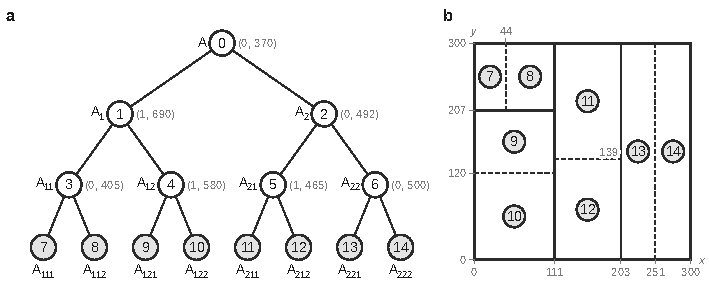
\includegraphics{figures/q38-partition-bsp.pdf}
\caption*{Figure 3 --- Exemple de creation(7) : (a) régions rangées en largeur, la
coupe i (direction, proportion) découpe la région i en 2i+1 et 2i+2 ;
(b) pavage du carré de côté 300 avec les coordonnées entières}
\end{figure}

\end{document}
